\section{Results}\label{sec:results}

This section presents the results of applying \texttt{GLaRe()} to our three motivating datasets --  the Glaucoma data (Section \ref{sec:glaucoma-reults}), the Proteomic Gels data (Section \ref{sec:gels-reults}) and the MNIST digits data (Section \ref{sec:mnist-reults}) -- to choose between our three built-in latent feature representation methods described in Section \ref{sec:learning-functions} -- Principal Components Analysis (PCA), the Discrete Wavelet Transform (DWT) and an autoencoder (AE).
For all three datasets, we use a tolerance level of $\epsilon = 0.05$ and cut-off criterion of $\alpha=0.95$ with hyperparatmeters and settings for the methods set at their defaults outlined in Section \ref{sec:learning-functions} unless otherwise specified.
Finally, in Section \ref{sec:sample-size-experiment}, we perform an experiment where we artificially decimate the sample size of the Glaucoma dataset to demonstrate the dependence of PCA and the DWT on different sample sizes.
Additional results of the case studies are presented in Appendix \ref{sec:additional-results}.

\subsection{Glaucoma Data}\label{sec:glaucoma-reults}

Figure \ref{fig:eye-results} displays the summary plot from the application of \texttt{GLaRe()} to the Glaucoma data.
PCA is the most suitable latent feature representation method for this dataset because it achieves the qualifying criterion at $K=41$, whereas DWT and AE do not achieve the qualifying criterion for $K \leq 261$.
A grid of equally-spaced values from $1$ to $261$ in increments of $10$ was used for the latent feature dimensions.
Although it was possible to use larger latent feature dimensions for the DWT and AE, the qualifying criterion was achieved for PCA at $K=41$ so it was deemed unnecessary.
The computation times for PCA, DWT and AE were $1.2$, $0.7$ and $69.4$ minutes, respectively.

\begin{figure}
    \centering
    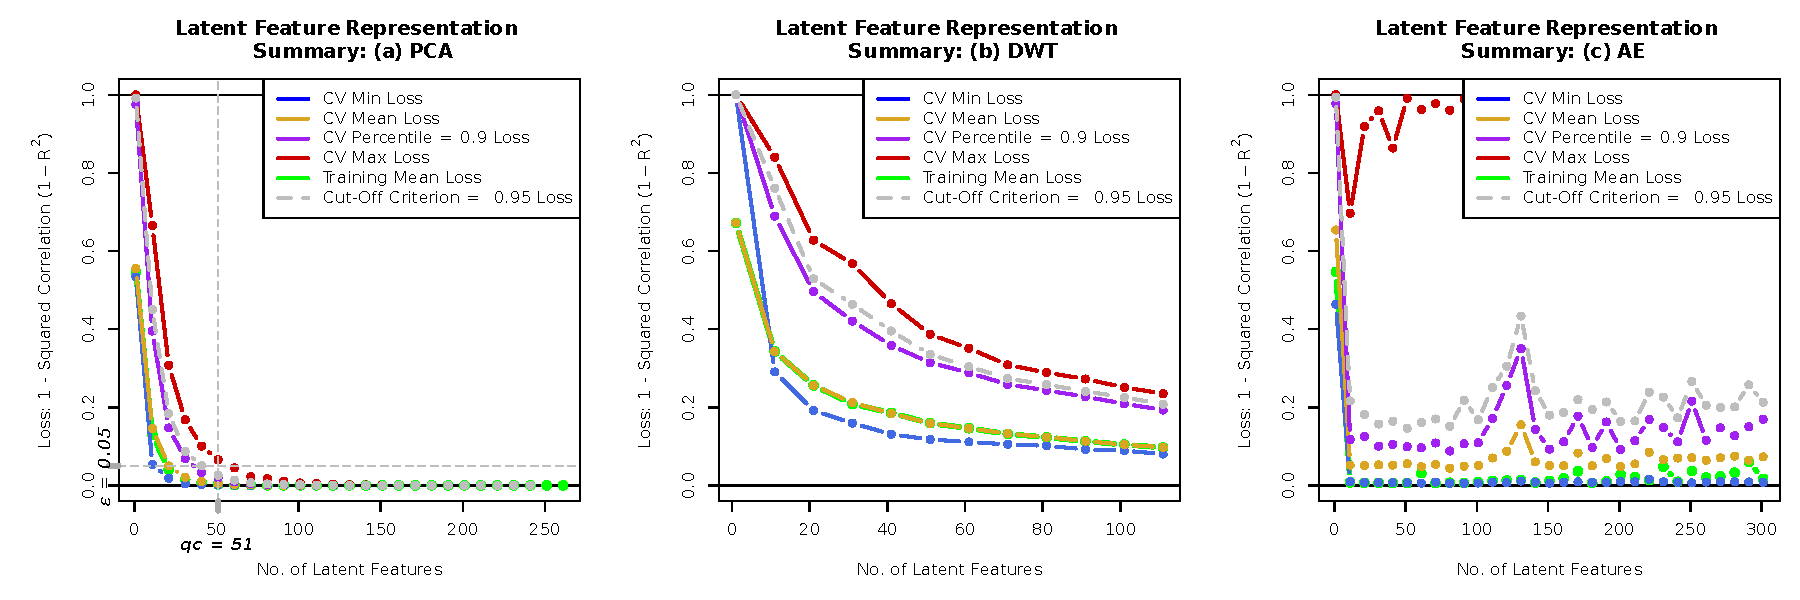
\includegraphics[width=1\textwidth]{figures/eye-results.pdf}
    \caption{Summary \texttt{GLaRe()} plot for the Glaucoma data. A grid of equally-spaced values from $1$ to $261$ in increments of $10$ was used for the latent feature dimensions.}
    \label{fig:eye-results}
\end{figure}

\subsection{Proteomic Gels Data}\label{sec:gels-reults}

\begin{figure}
    \centering
    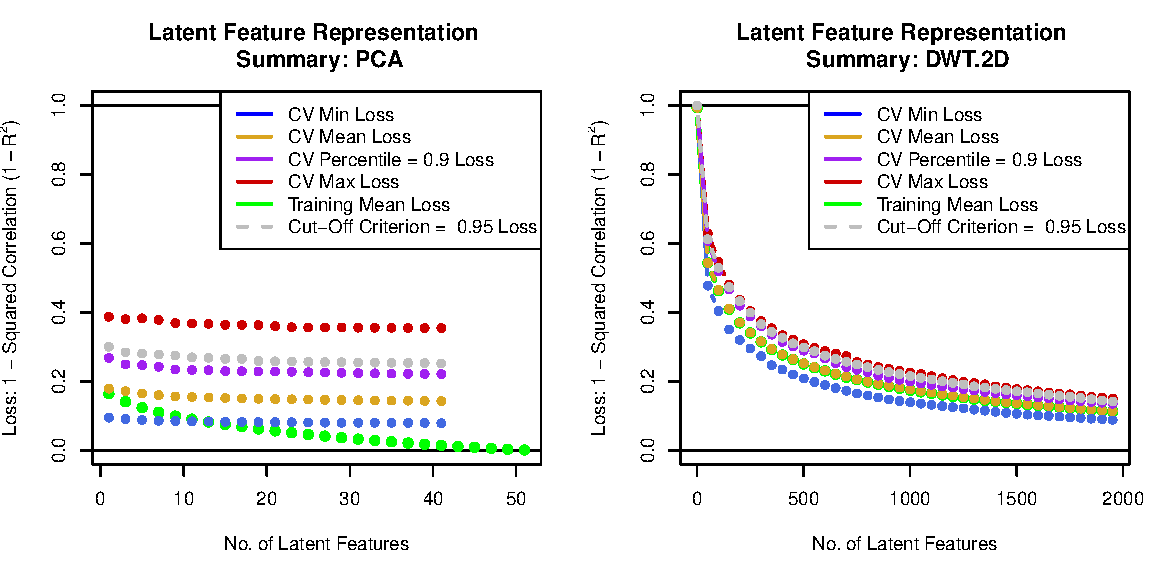
\includegraphics[width=1\linewidth]{figures/initial-gels.pdf}
    \caption{Preliminary results for the gels data.}
    \label{fig:enter-label}
\end{figure}


\subsection{MNIST Digits Data}\label{sec:mnist-reults}

Figure \ref{fig:mnist-results} displays the summary plot from the application of \texttt{GLaRe()} to the MNIST data.
PCA is the most suitable latent feature representation method for this dataset because it achieves the qualifying criterion at $K=201$, whereas DWT achieved it at $K=321$ and the AE did not achieve the qualifying criterion for $K \leq 381$.
A grid of equally-spaced values from $1$ to $381$ in increments of $20$ was used for the latent feature dimensions. 
The computation times for PCA, DWT and AE were $X_1$, $X_2$ and $X_3$ minutes, respectively.

\begin{figure}
    \centering
    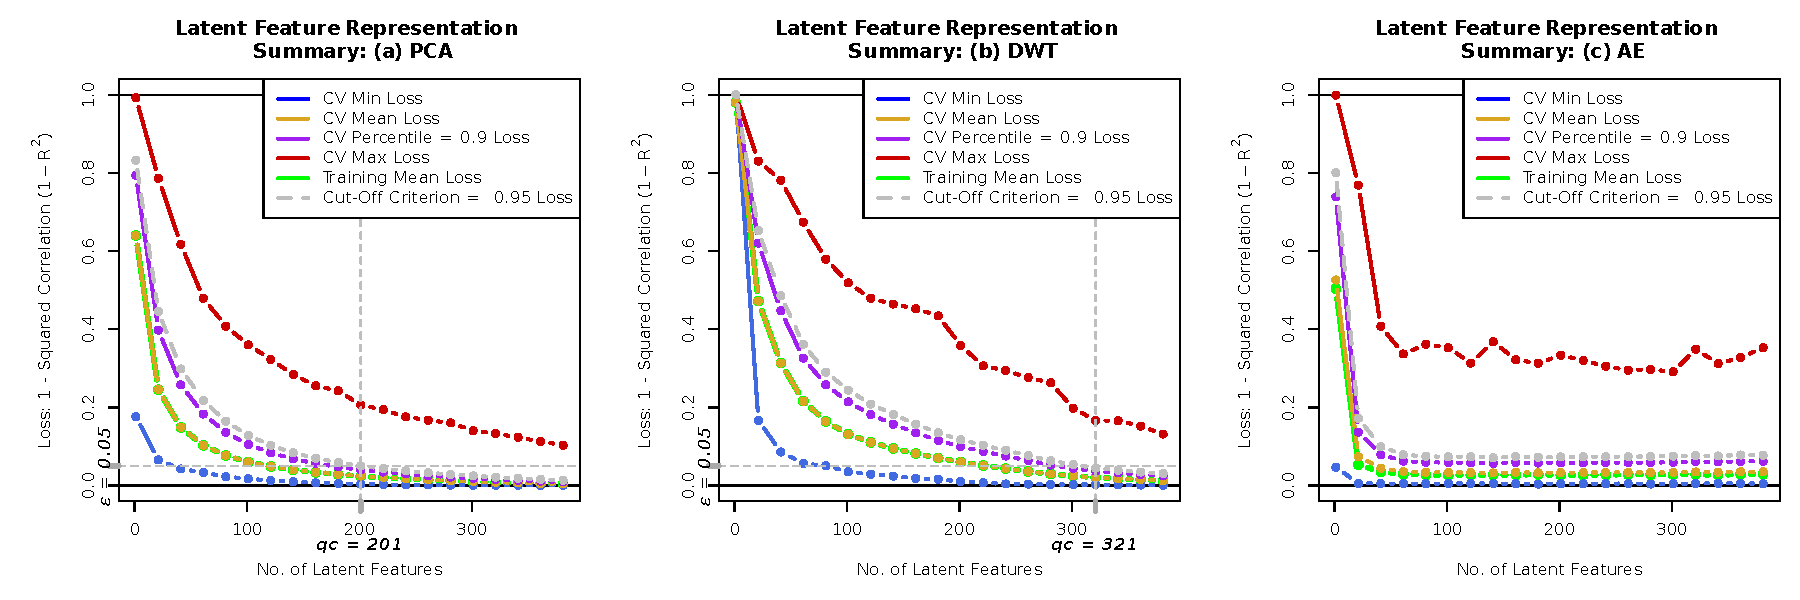
\includegraphics[width=1\textwidth]{figures/mnist-results.pdf}
    \caption{Summary \texttt{GLaRe()} plot for the MNIST data. A grid of equally-spaced values from $1$ to $381$ in increments of $20$ was used for the latent feature dimensions.}
    \label{fig:mnist-results}
\end{figure}

\subsection{Sample Size Experiment}\label{sec:sample-size-experiment}

In this section, we present the results of an experiment that demonstrates the dependence of flexible latent feature representation methods (e.g., PCA, AE) on sample size.
In PCA, the encoding and decoding transformations are learned entirely from the data, so it is highly dependent on having a sufficient sample size.
In contrast, the DWT transformation is fixed a-priori and for our thresholded wavelet representation only the \emph{ordering} of the wavelet coefficients to retain is learned from the data and hence there is less reliance on sample size.
We demonstrate this concept empirically on the Glaucoma dataset. We start with the full dataset ($N=606$) and then sub-sample the dataset to create smaller datasets of sizes $N=153$, $N=76$ and $N=38$ respectively.
We run \texttt{GLaRe()} using to compare the performance of PCA and the thresholded wavelet representation methods as the sample size is successively degraded.
In all cases, due to the small sample sizes, we use leave-one-out (rather than $k$-fold) cross-validation.

Figure \ref{fig:eye-sample-size-results-results-01} displays the results of our sample size experiment.
The PCA results are displayed in the first row and the DWT results are displayed in the second row.
As PCA can only estimate, at most, $\min(N-1, T)$ features and in this case $N<T$, we see that the maximum possible number of latent features changes as the sample size decreases.
In contrast, there is no restriction on the number of latent features for the DWT and we manually choose a maximum of $K=500$, which is sufficient to achieve the qualifying criterion (with $\epsilon=0.05$ and $\alpha=0.95$) in all four cases.
The greater reliance of PCA on sample size is reflected in Figure \ref{fig:eye-sample-size-results-results-01} in a number of ways.
Firstly, the displayed quantiles of the cross-validated loss distribution, in particular the maximum, $0.95$ and $0.9$ quantiles (red, grey and purple lines) increase noticeably for PCA as sample size is decreased, but they stay stable for the DWT.
The dependence is also reflected by the separation between the training and validation mean losses (green vs. yellow lines) as sample size is decreased, which demonstrates that PCA is unable to estimate a generalisable representation when the sample size is too small, even if the training mean loss is satisfactory.
Finally, we can achieve the qualifying criterion using the DWT in all four cases (albeit with fa large number of features), but we only achieve it for PCA with sample sizes $N=306$ and $N=153$.
In addition, the extra number of features needed achieve the qualifying criterion when the sample size is halved from $N=306$ to $N=153$ is slightly larger for PCA than the DWT: $qc=41$ to $qc=46$ for PCA vs. $qc=414$ to $qc=416$ for the DWT.
The experiment is subject to sampling variability induced in the sub-sampling stage, so we repeated the experiment using a different random seed and present the results in Appendix \ref{sec:additional-results}.

\begin{figure}
    \centering
    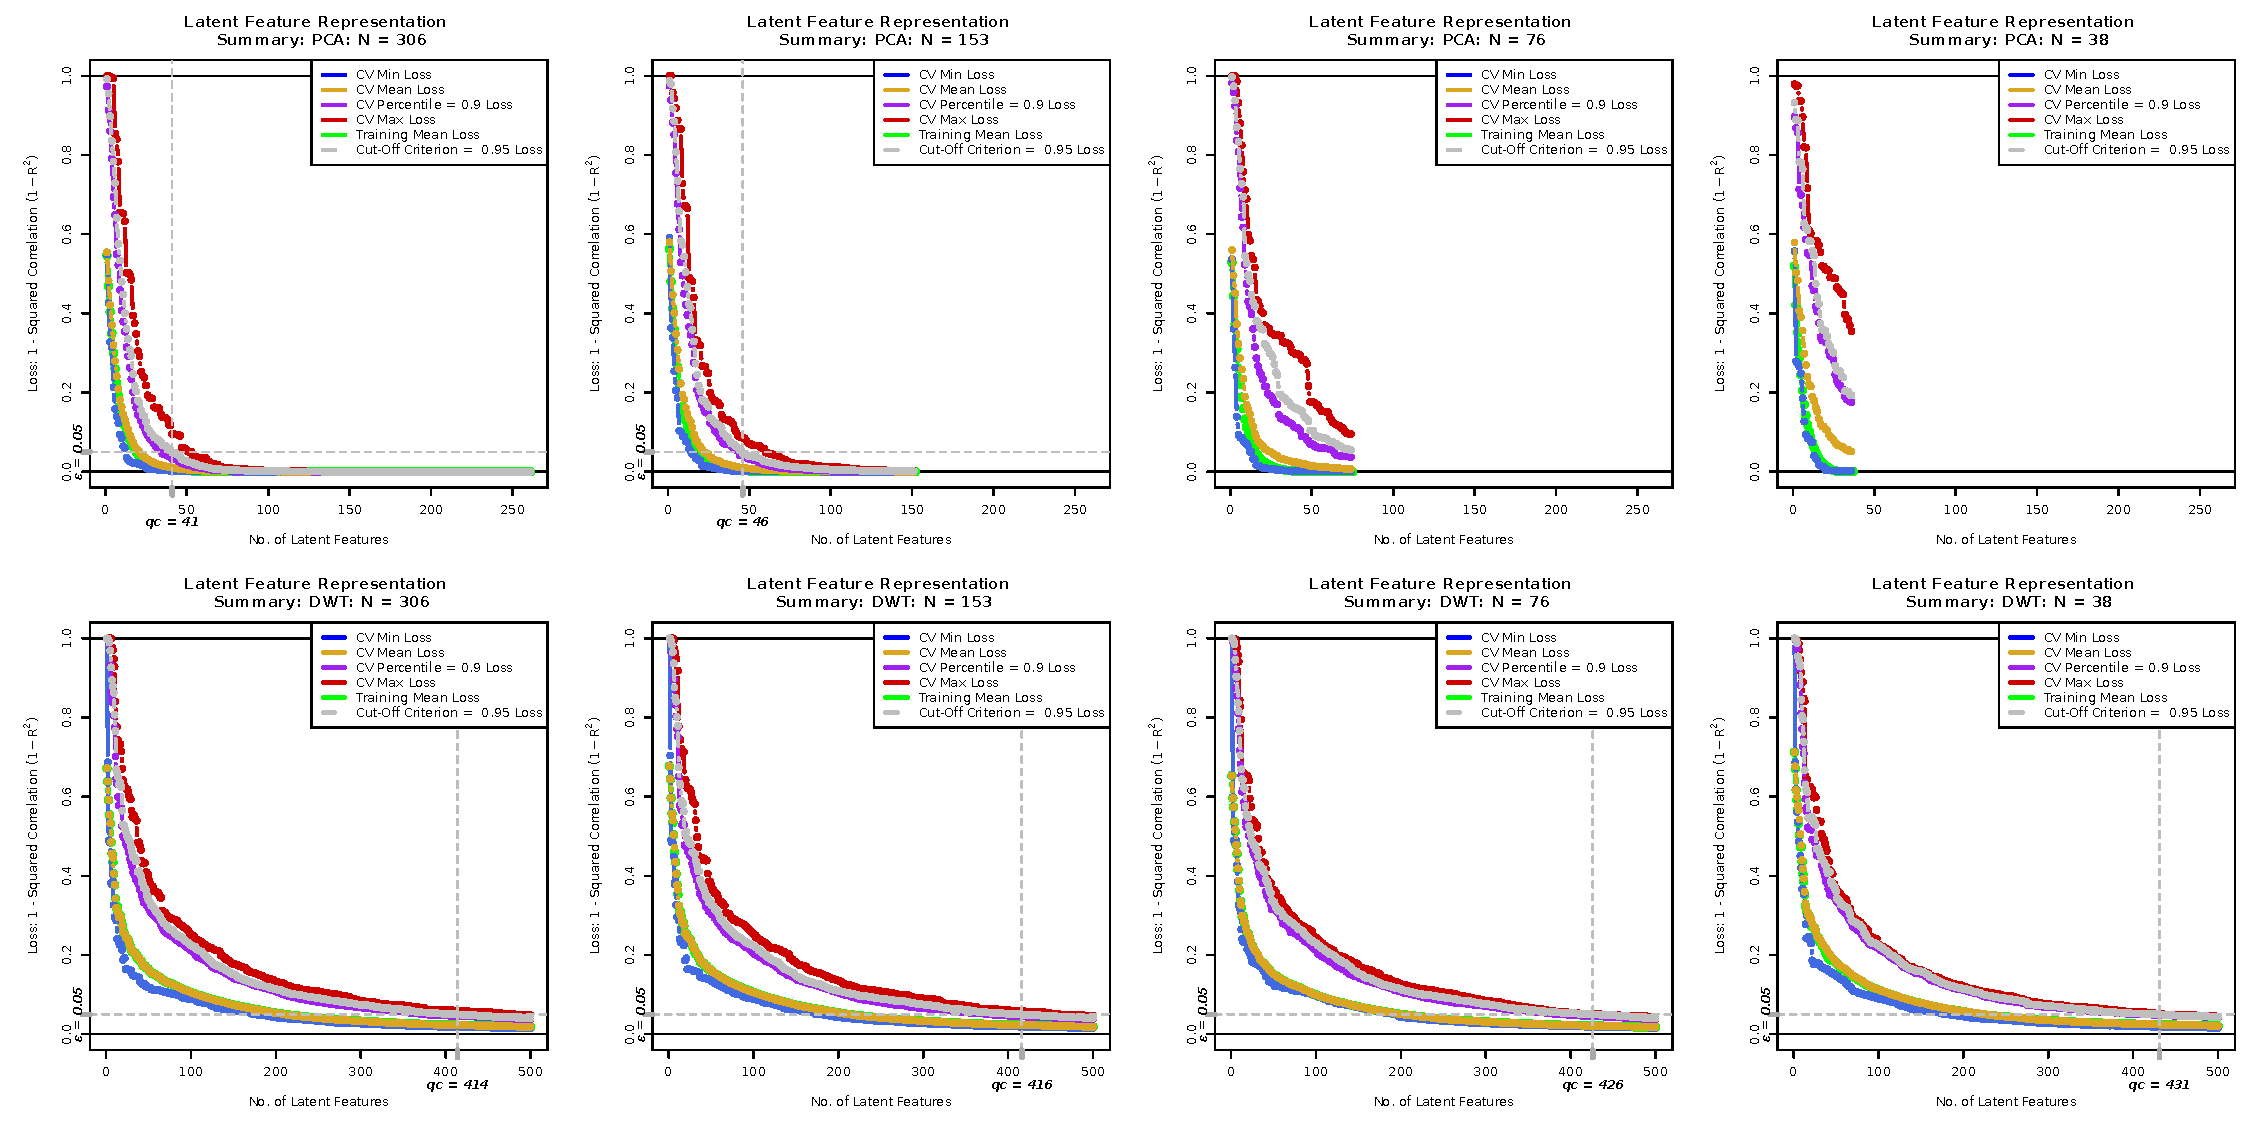
\includegraphics[width=1\linewidth]{figures/eye-sample-size-results-results-01.pdf}
    \caption{Results of the experiment to assess the affect of sample size on different latent feature representations. The Glaucoma data was used to create smaller datasets of size $N=153$, $N=76$ and $N=38$. \texttt{GLaRe()} was used to compare the representations provided by PCA (first row) and DWT (second row) as the sample size was decreased. Leave-one-out cross-validation was used in all cases.}
    \label{fig:eye-sample-size-results-results-01}
\end{figure}


